\chapter{Work Package Tasks}
\label{ch:wptasks}

In this chapter, we discuss in brief about the high level tasks in each WP. A reference architecture diagram is also given for each WP, this is meant to be seen as an early proposal and it is subjected to change in future documents.

\section{WP1: Service Descriptor Translator}

\subsection{Requirements definitions and architecture design}
\paragraph{}
The development of the SDT engine follows a microservice architecture. The architecture inludes a message broker with a subcriber/publisher model. The NSDs(yaml) corresponding to the communicating MANO are published to the broker. Our SDT engine, subscribed to the broker, consumes the yaml files and translate one MANO NSD to the other template and publish them back to the broker. These translated NSDs could be accessed by any other services through a REST API.
\begin{figure}[h]
	\centering
	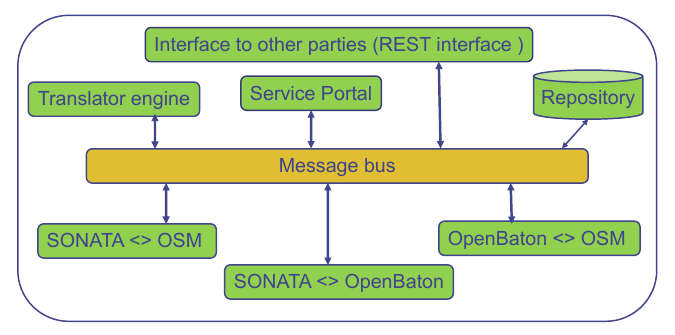
\includegraphics[width=0.9\linewidth]{figures/wp1Arch}
	\caption{Reference architecture for SDT}
	\label{fig:wp1arch}
\end{figure}

\subsection{Prototype implementation of SDT components}
\paragraph{}
After we plan the concrete architecture, we model a working prototype of the SDT engine including all the requisite components. This prototype is built as a standalone autonomous microservice.
\subsection{Proof of concept demonstration}
\paragraph{}
We demonstrate the functionality of our SDT engine on a virtual machine where atleast two different MANO frameworks are installed and deployed. 

\section{WP2: Service Descriptor Splitter}

\subsection{Requirements definition and architecture design}
\paragraph{}
We follow a publish/subscribe message broker model again for the SDS engine implementation. The NSD(yaml) is published to the message broker. A service graph splitter and a NSD splitter consumes the NSD from the broker and splits the NSD into two. The two seperate NSDs are published back to the broker from where other services can consume those through REST API.
\begin{figure}[h]
	\centering
	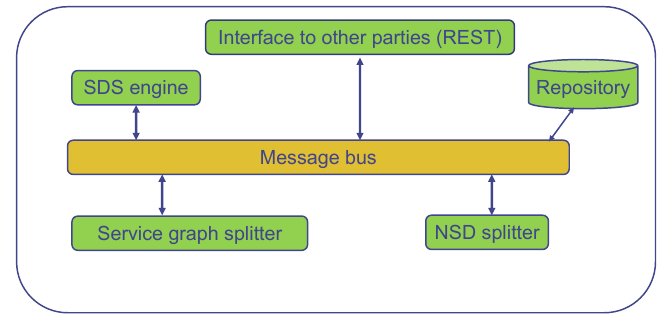
\includegraphics[width=0.9\linewidth]{figures/wp2Arch}
	\caption{Reference architecture for SDS}
	\label{fig:wp2arch}
\end{figure}

\subsection{Investigation of service graph partitioning algorithms and libraries}
\paragraph{}
The service graph needs to be split optimally based on the loads and resource allocation on each VNFs. To accomplish this we use a graph partitioning algorithm such as Mixed Integer Program for Partitioning Graphs. However the exact choice of algorithm suitable for our project will be decided as we progress.
\subsection{Prototype implementation of SDS components}
\paragraph{}
After we plan the concrete architecture, we code and model a working prototype of the SDS engine including all the requisite internal components. This prototype is also built as a standalone autonomous microservice.
\subsection{Proof of concept demonstration}
\paragraph{}
We demonstrate the functionality of our SDS engine on a virtual machine where atleast two different MANO frameworks are installed and deployed.

\section{WP3: MANO Adaptor}

\subsection{Requirements definition and architecture design}
\paragraph{}

\begin{figure}[h]
	\centering
	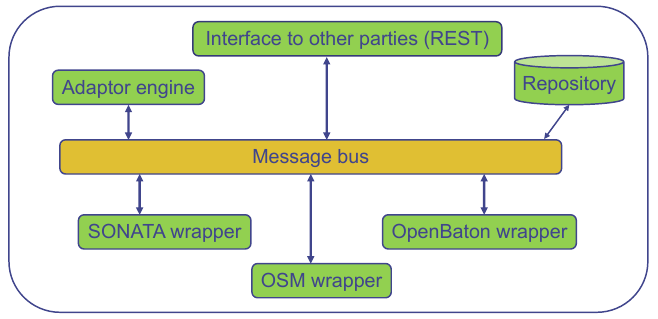
\includegraphics[width=0.9\linewidth]{figures/wp3Arch}
	\caption{Reference architecture for MA}
	\label{fig:wp3arch}
\end{figure}

\subsection{Prototype implementation of adaptor components}
\paragraph{}

\subsection{Investigation of MANO scalability challenges}
\label{wp3manoresearch}
The plan is to investigate MANO scalability challenges by answering research questions such as the ones listed below but not limited to. (Figure \ref{fig:wp3manoscale})
\begin{itemize}
	\item What is the optimal number of MANO instances in a system?
	\item What is the optimal hierarchical level in a system?
\end{itemize}

\begin{figure}[h]
	\centering
	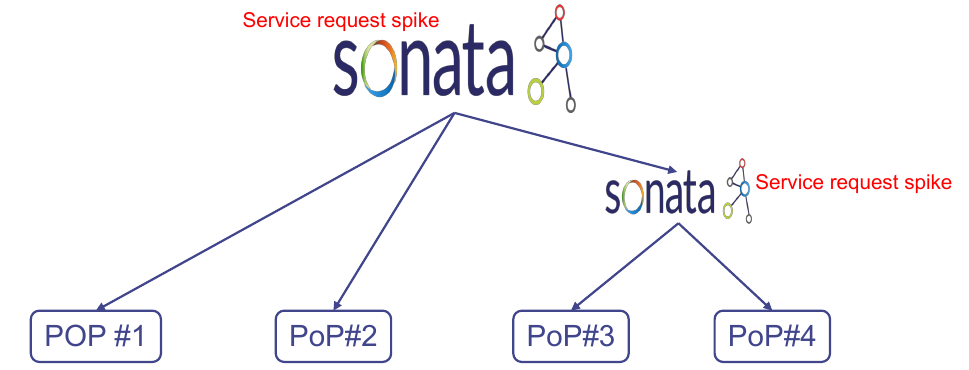
\includegraphics[width=0.9\linewidth]{figures/wp3manoScale}
	\caption{MANO scaling scenario}
	\label{fig:wp3manoscale}
\end{figure}



\subsection{Proof of concept demonstration}
